% !TeX spellcheck = cs_CZ
{\tikzset{external/prefix={tikz/APE/}}
 \tikzset{external/figure name/.add={ch02_}{}}
%================== Kapitola: Vlastnosti plošných spojů=============================================
\chapter{Vlastnosti plošných spojů}
\minitoc

  V této kapitole budou uvedeny některé důležité vlastnosti plošných spojů, potřebné pro
  správný návrh layoutu. Jedná se především o odpor, kapacitu, indukčnost a impedanci různých
  geometrických konfigurací vodičů a plošných spojů. Znalosti těchto vlastností jsou potom
  vstupní podmínkou pro úvahy o některých parazitních jevech na deskách plošných spojů a
  jejich eliminaci při návrhu (zpoždění průchodu signálu, odrazy na vedení, přeslechy, atd.).
  Veškeré vztahy uvedené v následujících kapitolách jsou čerpány z literatury 
  \cite[s.~55]{slyw038b}, \cite[s.~34]{Zahlava2005}, \cite[s.~34]{Ritchey2008}. Vztahy jsou ve 
  většině případů zjednodušené, což pro potřeby tohoto skripta postačuje, nebo
  cílem je ukázat, na jakých parametrech tyto vlastnosti závisí a ne vypočítat jejich přesnou
  hodnotu. Přesné výpočty přenechejme počítačovým simulačním programům.

\section{Odpor vodiče}
  Elektrický odpor je fyzikální veličina charakterizující schopnost elektrických vodičů vést 
  elektrický proud. Hodnota elektrického odporu je dána materiálem, tvarem i teplotou vodiče. 
  Velikost odporu závisí na délce vodiče (přímo úměrně), na obsahu průřezu vodiče (nepřímo úměrně), 
  na materiálu vodiče (měrný elektrický odpor) a na teplotě. Jelikož vodiče na deskách plošných 
  spojů mají obdélníkový průřez\footnote{při zanedbání změny tvaru při procesu leptání a pokovení}, 
  tak jak je znázorněno na obr. \ref{ape:fig001}, můžeme hodnotu odporu vodiče stanovit podle 
  známého vzorce
  \begin{equation}\label{ape:eq001}
    R_{\vartheta_0} = \varrho\dfrac{l}{S} = \varrho\dfrac{l}{t\cdot w} \qquad[\si{\ohm}]
  \end{equation}
  kde \(\varrho\ldots\) \emph{měrný elektrický odpor} [\si{\ohm\m}], \(l\ldots\) \emph{délka 
  vodiče} [\si{\m}] a \(S\ldots\) \emph{průřez vodiče} [\si{\m\squared}]. Symboly \(t\) a \(w\) 
  odpovídají kótování z obrázku \ref{ape:fig001}.
  
  
  \begin{figure}[ht!] %\ref{ape:fig001}
    \centering
    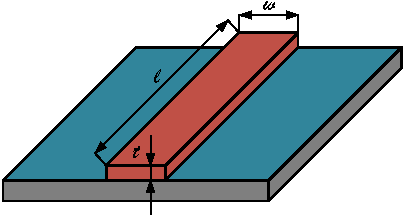
\includegraphics[width=0.7\linewidth]{ape_fig001.pdf}
    \caption{Odpor vodiče plošného spoje
             (\cite[s.~34]{Zahlava2005})}
    \label{ape:fig001}
  \end{figure}

  Závislost odporu na teplotě je dána vztahem \cite[s.~24]{Necasek1972} 
  \begin{equation}\label{ape:eq002}
    R_\vartheta = R_0\cdot[1+\alpha(\vartheta - \vartheta_0)] \qquad[\si{\ohm};\si{\ohm}, 
    \si{1\per\degreeCelsius}, \si{\degreeCelsius}]
  \end{equation}
  kde \(\alpha\ldots\) \emph{teplotní odporový součinitel}, \(R_\vartheta\ldots\) výsledný odpor 
  teplého vodiče,  \(R_{\vartheta_0}\ldots\) odpor vodiče při výchozí teplotě, \(\vartheta\) 
  (theta) výsledná teplota, \(\vartheta_0\) výchozí teplota (teplota okolí).
  
  Oteplení 
  \begin{equation}\label{ape:eq003}
    \Delta\vartheta = \vartheta - \vartheta_0 \qquad[\si{\degreeCelsius}; \si{\degreeCelsius}]
  \end{equation}
  
  Konečná teplota
  \begin{equation}\label{ape:eq004}
    \vartheta = \vartheta_0 + \Delta\vartheta \qquad[\si{\degreeCelsius}; \si{\degreeCelsius}]
  \end{equation}

\section{Skin efekt}
\section{Kapacita vodiče}
\section{Indukčnost vodiče}
\section{Impedance}
\section{Rychlost šíření signálu}
\section{Vliv kapacitní zátěže}
\section{Přeslechy}

\section{Zatížení vodičů na plošném spoji}
  Při návrhu plošných spojů je nutné znát jejich proudovou a napěťovou zatížitelnost. Při
  vysokém proudovém zatížení může dojít vlivem ztrátového výkonu na odporu plošného
  vodiče k jeho nadměrnému zahřátí a dokonce až k přetavení. Napěťová zatížitelnost souvisí
  s elektrickou pevností izolačních mezer mezi vodiči na plošném spoji.
  
  \subsection{Proudové zatížení}
    Proudová zatížitelnost plošných spojů je neobyčejně velká, neboť v porovnání s drátovým
    vodičem má plošný spoj daleko vetší ochlazovací plochu. 
    
    Pro vytvoření pravidel pro individuální návrh plošných spojů s ohledem na přenos proudu lze 
    postupovat podle průmyslového standardu \textbf{IPC-2152}: (Standard for Determining 
    Current-Carrying Capacity in Printed Board Design).  

    \begin{figure}[ht!] %\ref{ape:fig002}
      \centering
      \begin{tabular}{c}
       \subfloat[ ]{\label{ape:fig002a}
         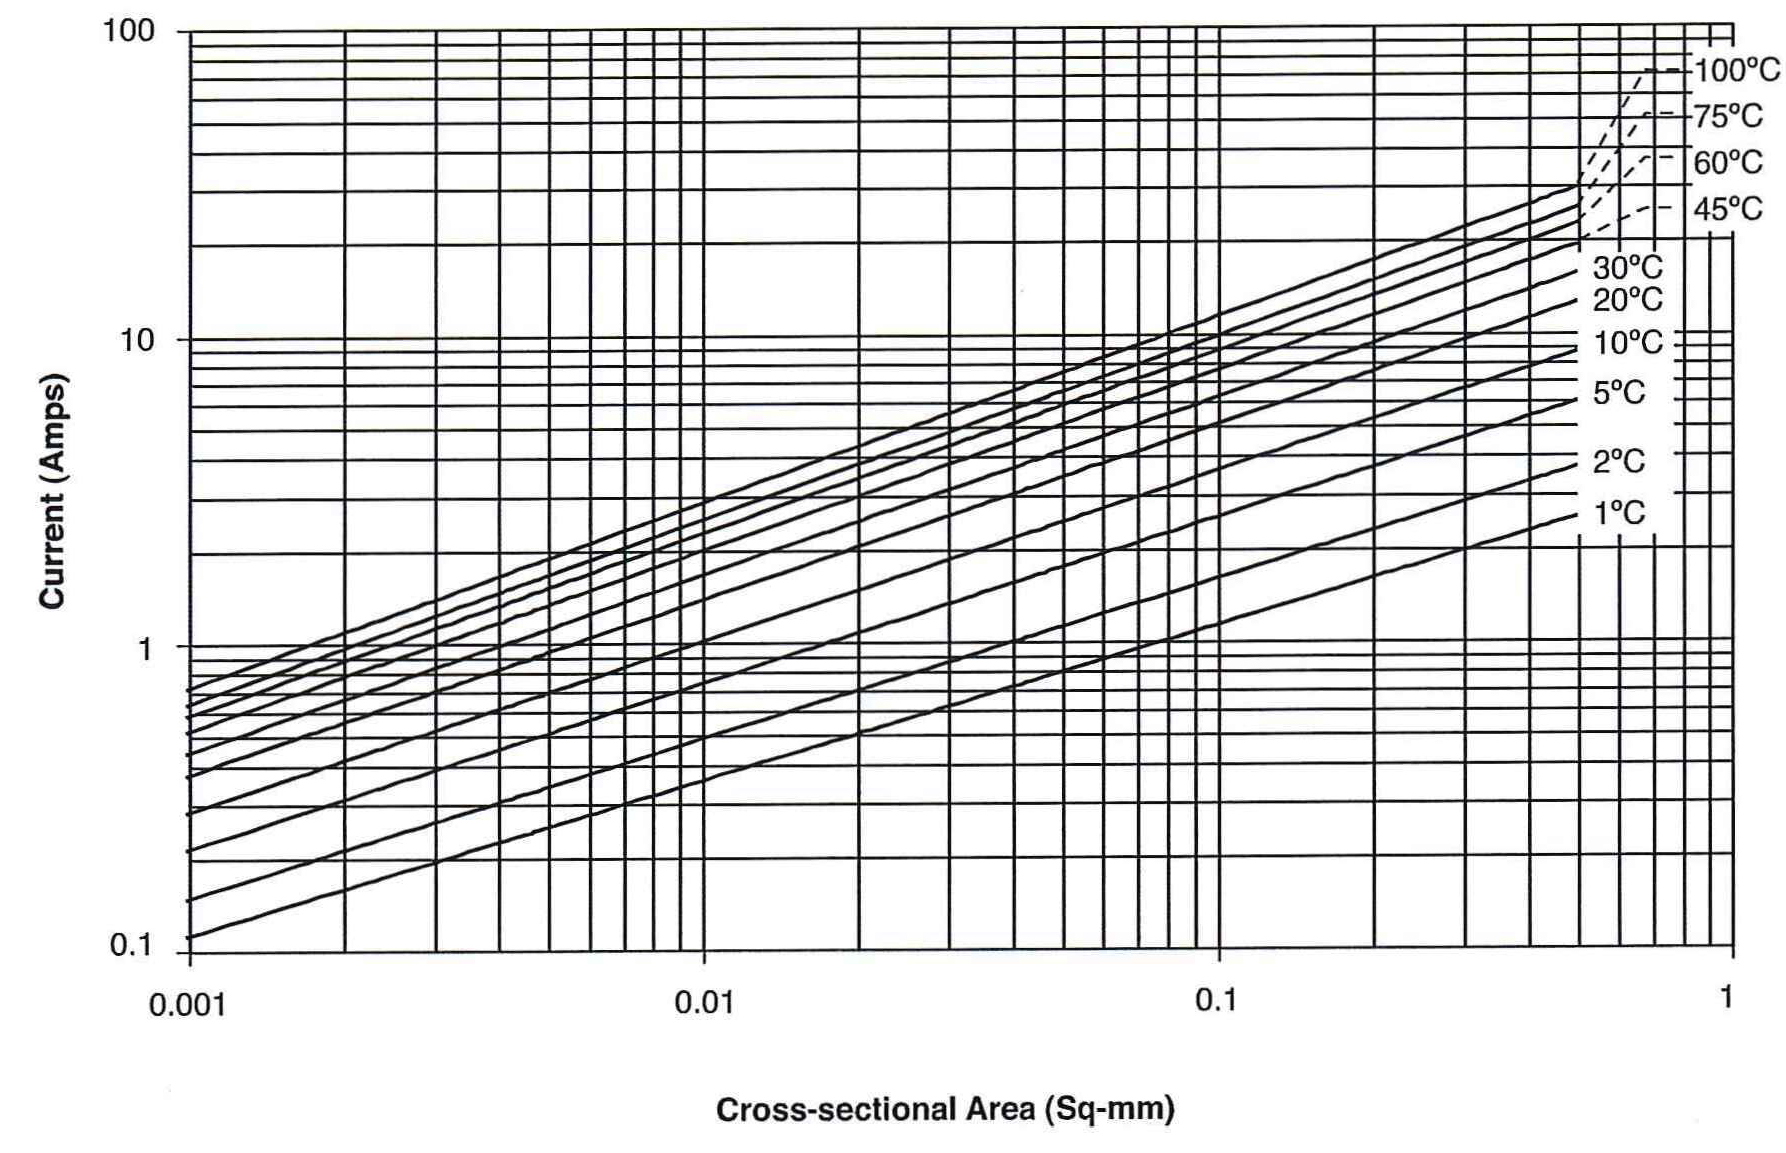
\includegraphics[width=1\linewidth]{ape_fig002a.png}} \\
       \subfloat[ ]{\label{ape:fig002b}
         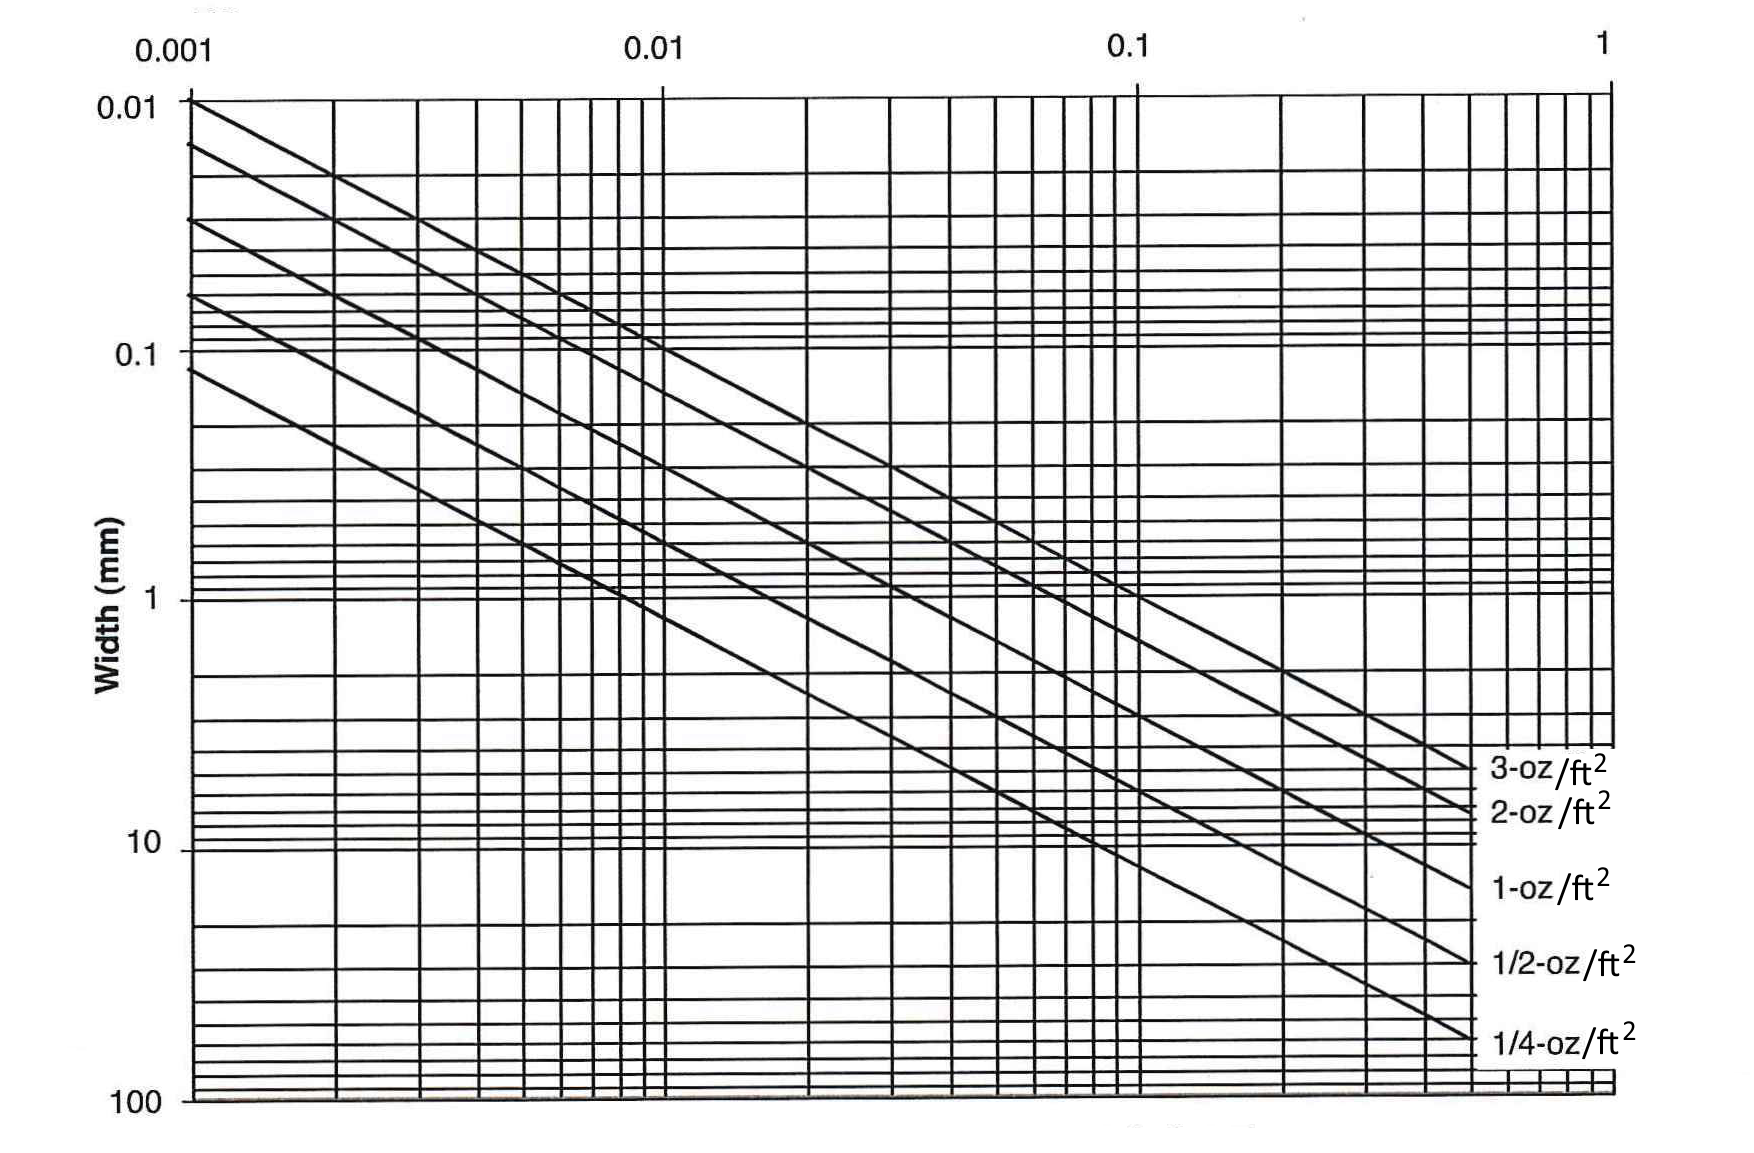
\includegraphics[width=1\linewidth]{ape_fig002b.png}}
      \end{tabular}
      \caption{a) Křivky závislosti stejnosměrné proudové zatížitelnosti na průřezu plošného spoje 
               pro různé oteplení; b) Graf pro určení průřezu spoje pro danou šířku a tloušťku 
               plátované měděné fólie.
               (\cite[s.~9]{IPC2152}).}
      \label{ape:fig002}
    \end{figure}
    
    Například pro spoj s průřezem \SI{0.1}{\mm\squared} a oteplení \SI{100}{\degreeCelsius} 
    dostaneme proudovou hustotu \SI{100}{\A\per\mm\squared} (viz graf \ref{ape:fig002a}). Maximální 
    provozní teplota je dána takzvaným bodem měknutí základního materiálu, který je u \texttt{FR4} 
    \SI{125}{\degreeCelsius}. 
    
   
    \begin{figure}[ht!] %\ref{ape:fig003}
      \centering
      \begin{tabular}{c}
       \subfloat[pro průřez vodiče od \SI{0.1}{\mm\squared} do       
       \SI{0.5}{\mm\squared}]{\label{ape:fig003a}
         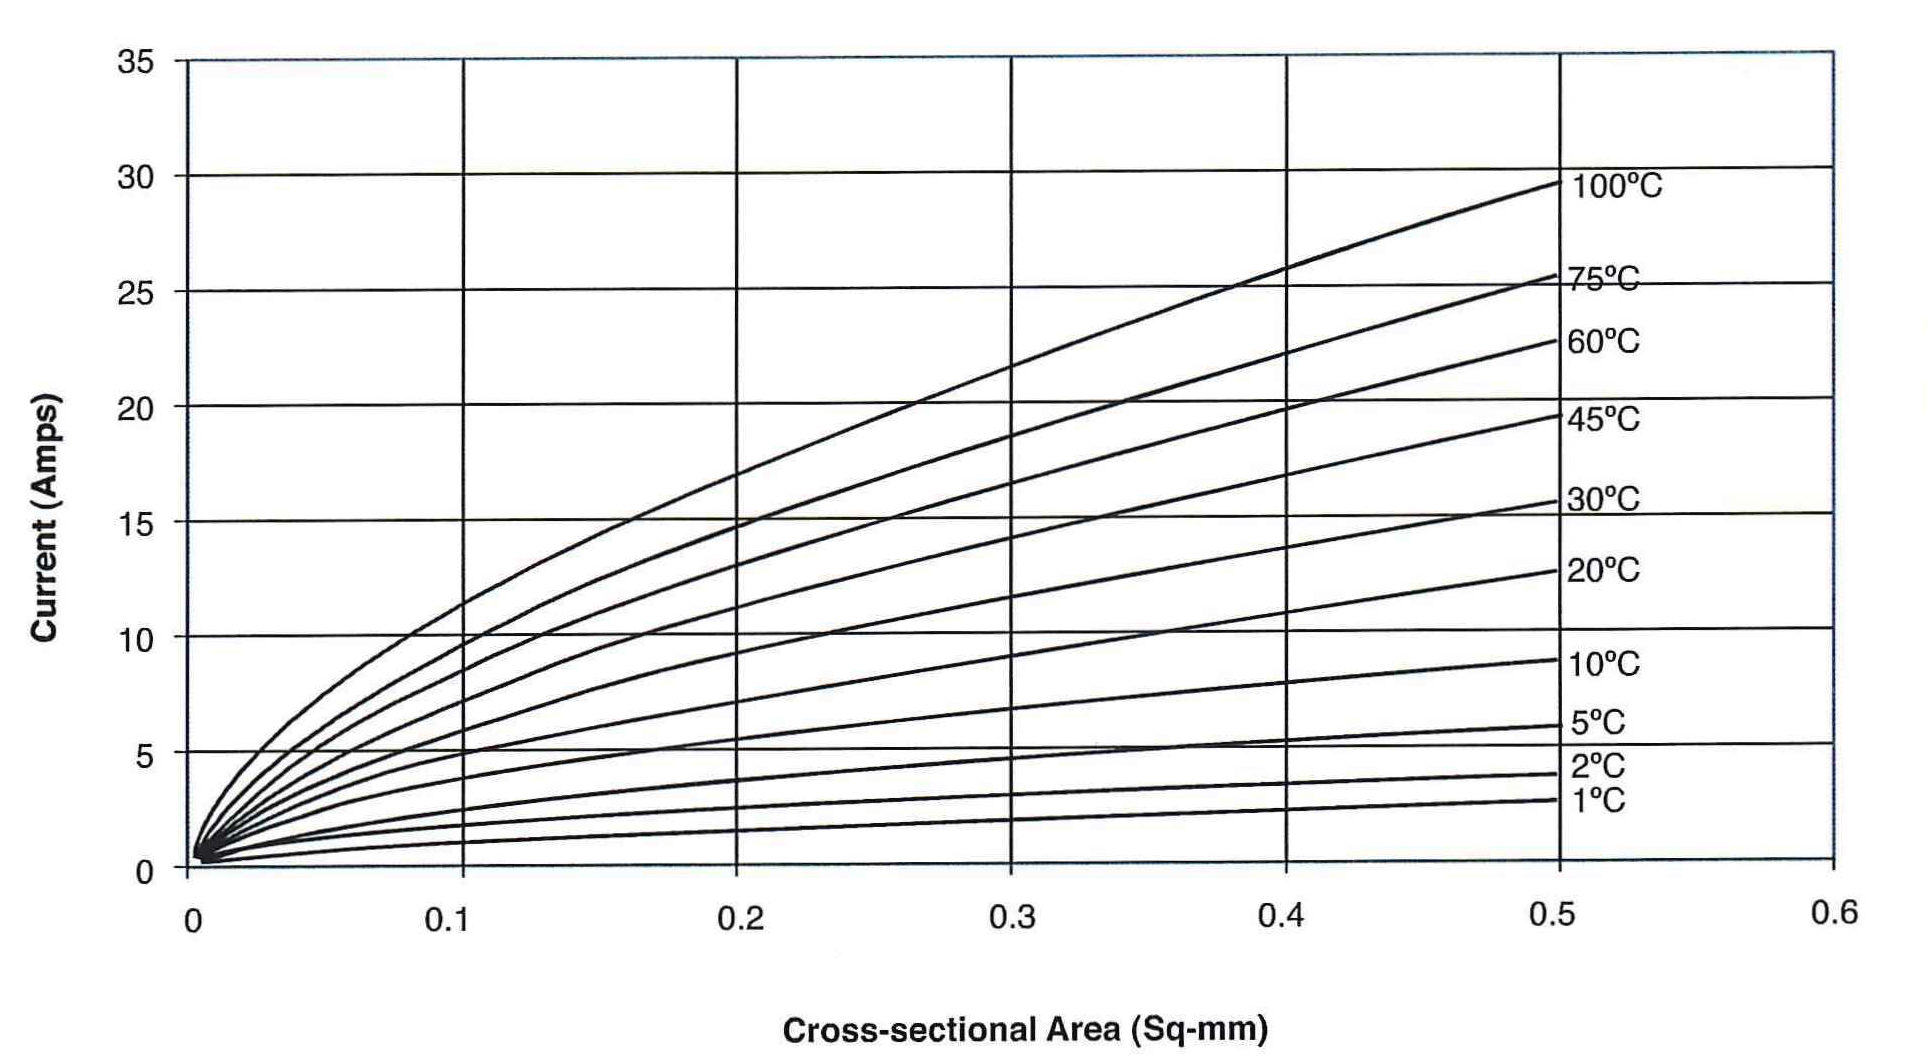
\includegraphics[width=1\linewidth]{ape_fig003a.png}} \\
       \subfloat[Závislost pro průřez vodiče od \SI{0.01}{\mm\squared} do
              \SI{0.1}{\mm\squared}]{\label{ape:fig003b}
         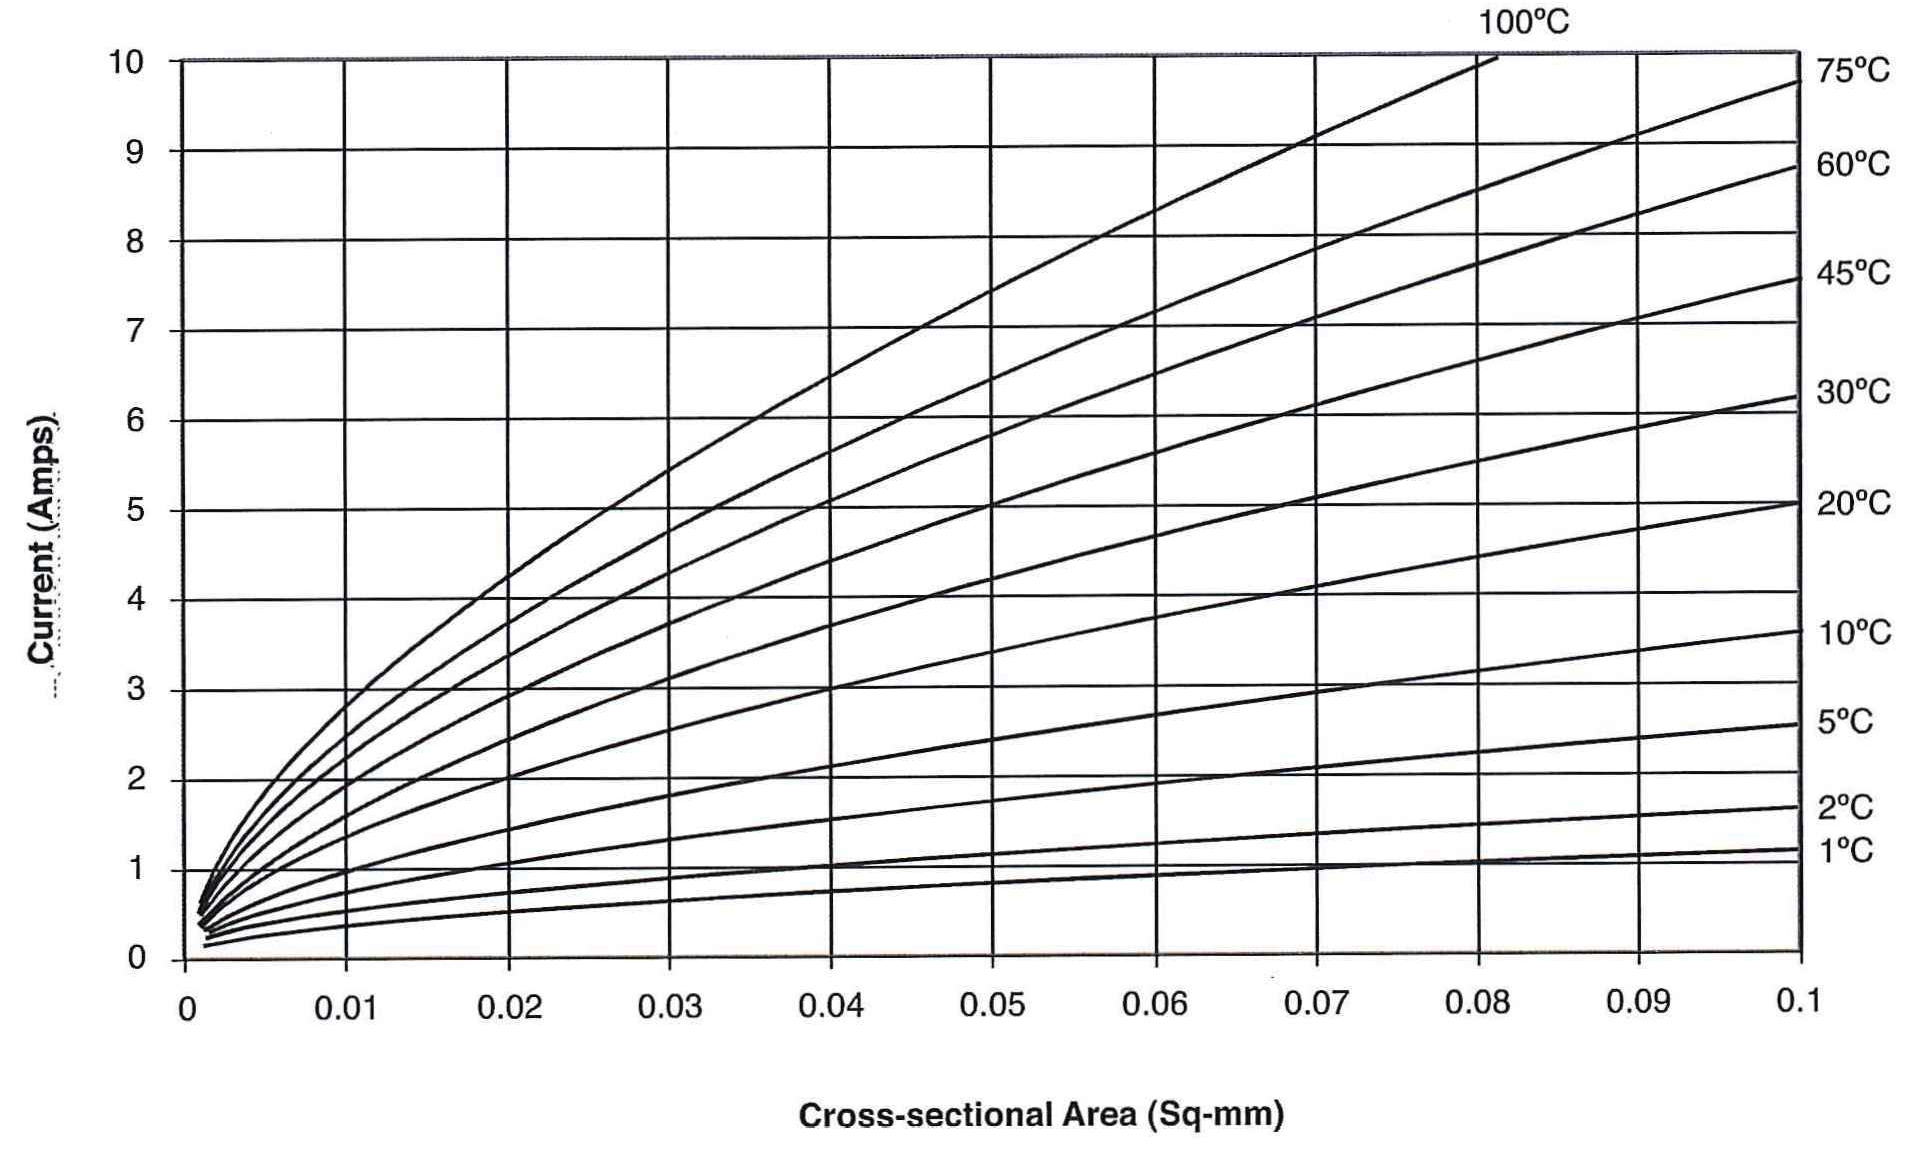
\includegraphics[width=1\linewidth]{ape_fig003b.png}}
      \end{tabular}
      \caption{Křivky závislosti stejnosměrné proudové zatížitelnosti na průřezu plošného spoje 
                pro různé oteplení
               (\cite[s.~10]{IPC2152}).}
      \label{ape:fig003}
    \end{figure}

    Stupeň ohřátí plošného vodiče vlivem průchodu elektrického proudu závisí na odporu vodiče,
    velikosti a době průchodu proudu a možnostech odvodu tepla. Proudové přetížení má za
    následek nejen zhoršení adheze vodiče k základnímu materiálu účinkem vyvinutého tepla, ale
    také vznik značných mechanických sil vlivem průtoku proudu a tepelné dilatace. 
    
    \begin{example}
      Požadovaný protékající proud je \SI{8}{\A} s maximálním teplotním nárůstem 
      \SI{30}{\degreeCelsius}. Jak široký vodič je nutné použít, má-li deska \SI{35}{\micro\m} Cu 
      fólii (\num{1} \(oz/ft^2\))? 
      
    \end{example}
    
  \subsection{Napěťové zatížení}
    Velikost přípustného napětí mezi vodiči závisí na mnoha faktorech. Jsou to například velikost
    mezery, druh základního materiálu, ochranný povlak (nepájivá maska), vlastnosti prostředí a
    v neposlední řade provozní a předepsané bezpečnostní požadavky. Ochranný povlak přispívá
    k zachování vlastností desky s plošnými spoji, je-li vystavena působení nepříznivých vlivu
    jako je prach a vlhkost. Rozlišujme průrazné napětí a maximální provozní napětí. Velikosti 
    těchto napětí a způsoby jejich zkoušení jsou předmětem norem. 

} %tikzset
%---------------------------------------------------------------------------------------------------
\printbibliography[title={Seznam literatury}, heading=subbibliography]
\addcontentsline{toc}{section}{Seznam literatury}